%%
%% GENERAL INSTRUCTIONS
%%
%% Each team member should contribute to the writing/editing of each section.
%%
%% Replace the \section titles with specific phrases related to your project.
%%
%% You may rearrange the order as long as you address the main prompts below.
%%

\documentclass[11pt]{article}

\usepackage{graphicx}

% fonts
\usepackage[utf8]{inputenc}
\usepackage[T1]{fontenc}
\usepackage[sc]{mathpazo}

% spacing
\usepackage[margin=1in]{geometry}
\setlength{\parskip}{1ex}
\usepackage{multicol}
\usepackage{setspace}
\onehalfspacing

% orphans and widows
\clubpenalty=10000
\widowpenalty=10000

%------------------------------------------------------------------------------%
\begin{document}

%% Insert the name of your project, the name of your team, and the name and email of each student.

\begin{center}
\bfseries\huge
Post Office Database Proposal
\end{center}

\begin{center}
\itshape\large
Postalrific
\end{center}

\begin{multicols}{4}
\centering

John Button \\
{\footnotesize buttonjh@dukes.jmu.edu}

Parth Parikh \\
{\footnotesize parikhpb@dukes.jmu.edu}

Jacob Campbell \\
{\footnotesize campbejs@dukes.jmu.edu}

Jacob Bringham \\
{\footnotesize bringhja@dukes.jmu.edu}

\end{multicols}

%------------------------------------------------------------------------------%
\section*{Problem and Vision}

%% Introduce the main idea of your project. What is the exact problem you are going to solve? What is your vision for the solution? How will this benefit potential stakeholders? (e.g., users, data owners, society) Provide background information about the problem domain.

United States Postal Service (USPS) locations provide important services for many communities across the country, especially under-served communities that may be unprofitable for private businesses to provide postal services for. Although Congress appropriates funding for USPS, the decisions to open and close post offices is left to USPS itself and a Postal Regulatory Committee. Although there are some guidelines regarding protecting rural communities from post office closures, there is no set policy as to which communities will be serviced and which will not be. USPS holds the ultimate authority to close locations, regardless of local or state level consultation. 

Our group believes it is important to look at this important public data to ensure that USPS resources are being distributed equitably across income levels, racial groups, and political boundaries. This project will compare US Census data with USPS office locations within Virginia in order to determine if there are under-served or over-served counties and communities. By comparing this data, it may be useful for policymakers to understand where USPS resources may be redistributed to service Virginians better. It may also be useful to decide which areas may be over-served if policymakers decide to cut back USPS appropriations, a popular idea in recent years amongst those who wish to cutback government spending. 

%------------------------------------------------------------------------------%
\section*{Data and Questions}

%% Describe the data sets you will use. Where does the data come from, and who owns it? What is the data primarily about? About how much data is available? Include several example rows/instances to illustrate what the data looks like.

%% Discuss two or three specific questions about the data that your project will answer. How are these questions interesting? Why are they important questions to answer? What resources already exist that help answer these questions?

For this project our information on post offices came from the Harvard Dataverse. We will be utilizing the county's the post office are located in VA as well as the name and start date. We are also thinking about incorporating the population density of each county into our data sets. As you can see in the table below, our data is primarily focused on post offices located in Virginia and whether they are equally distributed within the state. As of now, there is a lot of information about post offices in the United States. As a result, we are narrowing our search to only the ones within the state of Virginia. When referring to the data, you will also notice information about when the office was established and discontinued. One more thing the second picture illustrates, are the coordinates we will be utilizing in order observe which counties are under served in the state of Virginia. 

One of the main questions our data will answer is whether different counties in the state have equal access to the United States Postal Service. It will also provide a convenient way for individuals who are searching for homes and need access to a postal service that is within their range. It will allow future homeowners to make educated decisions on their accessibility through the postal services for collecting, processing, and transmitting mail. Finally, it will also provide information about which post offices are still in commission today. The reason these questions are important for us to answer is because it allows us to see changes within a community and provide aid in terms of future development.

% NOTE: I changed the graphic to cut out the GNIS columns so we didn't have to explain them in the proposal.
\begin{center}
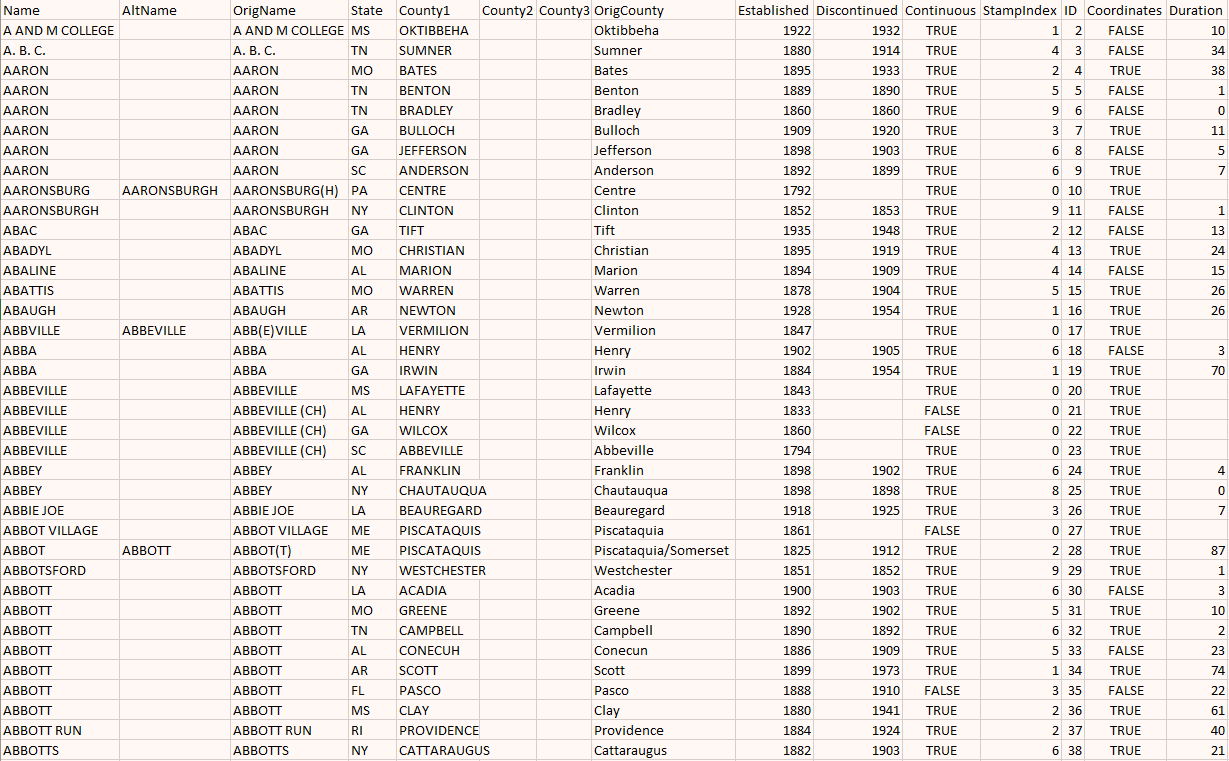
\includegraphics[width=1.0\linewidth]{sample.PNG}
\par
\end{center}

Above is a snippet of the data from the Harvard Dataverse. It contains information about various post offices such as their name, state and county within Virginia. Information such as longitude and latitude is also included.
% END JAKE CHANGES
%------------------------------------------------------------------------------%
\section*{Users and Specs}

%% Describe the main users of your application. Be specific; for example, what is their profession? How much experience do they have with data? Why would they want to use your project?

%% Discuss the high-level specifications. What functionality will your completed application provide? Explain a few use cases: what the user will do, and what the app will do. Leave out the technical details, such as what programming languages and software tools you'll use.

We have identified two groups of users who would be the target audience of out application. The first group is the average citizen of Virginia. The citizen can use our application to see if their current community is being serviced properly by the USPS compared to other counties in Virginia. A citizen could also use our application as a way to aid in moving to a new location in Virginia, as they can see if their prospective home is near USPS offices. The second group of users we have identified are government officials and policy makers. Our application can aid in identifying under serviced or over serviced communities. This allows them to propose changes to the USPS offices to better serve their community.

A use case for the first group of users, an average citizen looking to move to a location in Virginia would be: Identify the county and the application will return the number of USPS offices, their names, IDs, Coordinates, and county population. Another would be: Identify all the counties of Virginia to see the whole state's number of USPS offices and their information. Furthermore, they could identify decommissioned offices to see the history of USPS offices in Virginia. 

A use case for the second group of users, a policy maker would be: specify county, population, and proportion of minority status to see if certain counties are being serviced based on race. The application would supply them with the offices in that county and population of the county. The data can be used to aid them in deciding if there are parts of the state that are not being reached as readily. 

%------------------------------------------------------------------------------%
\section*{About the Team}

%% Include a short biographical sketch for each team member. Focus on academic and professional experience, not where you were born and what your hobbies are. For example, you might list the most recent/advanced CS courses you have completed, software projects you have worked on the in past, internships or other relevant work experience, and/or unique background abilities and skills that you will bring to the project.

John Button has recently completed college courses in Data Structures and Software Engineering. John has only completed one software project within his software engineering course, although he has worked on teams building products before during his cybersecurity internship in the telecommunications industry. John also takes history courses for his minor, giving him experience with analyzing primary sources and data while also taking in account real world context.

Parth Parikh has completed numerous computer science courses at James Madison University including Computer Systems 2 and Programming Languages. He has also completed the Software Engineering course where he gained hands-on experience working with other team members through Agile development. This was his first time working on a project with other individuals where they had to meet certain deadlines to please their client. With his skills and experience, he was able to earn an internship over the summer working for Peraton as a Software Engineer. Not only that, but he will also assist with the front-end development on representing the database to the user.   

Jacob Campbell has completed Data structures and Algorithms, Web Development, and Computer Systems 2. He has experience working in a group environment utilizing the Agile framework. He created a stock trading bot using API calls as a personal project. This project was key in getting him an internship last summer at Inadev as a Full Stack Developer intern. He studied Angular and Natural Language Processing using pythons NLTK library. Working in a professional environment gave him an insight of what would be expected of developers in industry.

Jacob Bringham has recently completed Programming Languages, Discrete Structures II and Artificial Intelligence. He has worked with teams of software developers both in school and at his internship with Sedna Digital Solutions (subcontractor of Lockheed Martin). He has designed and developed software to automate the testing of US Navy Systems. His skills gained from 3 years at JMU combined with work experience will make him a valuable part of the team.
%------------------------------------------------------------------------------%
\end{document}
